% !TeX spellcheck = de_DE
\documentclass{uebung_cs}
\usepackage{algo121}
\blattname{Wochenplan: Gierige Algorithmen}

\begin{document}
\section*{Vorbereitung}
Lies E Kapitel 4 und schau das Video der Woche.

\section*{Dienstag}
\begin{aufgabe}[Dateien auf Band]
    Auf einem Magnetband sind $n$ Dateien gespeichert.
    Die Längen der Dateien sind durch ein Feld $L[1..n]$ gegeben, das heißt, die $i$-te auf dem Band gespeicherte Datei hat Länge $L[i]$.
    Um Datei $k$ zu lesen, muss das Band alle Dateien von $1$ bis $k$ lesen.
    \begin{enumerate}
        \item(\warmup) Betrachte ein Band, auf dem sechs Dateien mit $L=[8,3,1,6,4,2]$ gespeichert sind. Zum Beispiel hat Datei $1$ die Länge $8$.
        Wie hoch sind die Kosten, um Datei $4$ zu lesen?
        \item(\warmup) Wie hoch sind die erwarteten Kosten bei a), wenn ein sechsseitiger Würfel geworfen wird und die damit indizierte Datei gelesen wird?
        \item Wenn jede Datei $k$ mit Wahrscheinlichkeit $1/n$ angefragt wird, sortieren wir die Dateien am Besten der Größe nach. Jetzt aber sind manche Dateien beliebter als andere: Datei $k$ wird mit Wahrscheinlichkeit $F[k]$ angefragt. Das heißt, $F[1..n]$ ist eine Wahrscheinlichkeitsverteilung über $\{1,\dots,n\}$ und die erwarteten Kosten sind
          \[\sum_{k=1}^n \sum_{i=1}^k F[k]\cdot L[i]\,.\]
        In welcher Reihenfolge müssen wir die Dateien jetzt sortieren, damit die erwarteten Kosten so klein wie möglich sind?
    \end{enumerate}
\end{aufgabe}

\begin{aufgabe}[Huffman-Codierung]
    Betrachte das Alphabet $\{\texttt a,\dots,\texttt g\}$ mit der folgenden Häufigkeitstabelle:
	\begin{center}
		\begin{tabular}{ccccccc}
			\texttt{a}&\texttt{b}&\texttt{c}&\texttt{d}&\texttt{e}&\texttt{f}&\texttt{g}\\\hline
			3&3&1&1&7&2&4\\
		\end{tabular}
	\end{center}
    \begin{enumerate}
        \item Führe den Algorithmus zur Huffman-Codierung für diese Häufigkeitstabelle aus und gib jeden Zwischenschritt an.
        \item Gib einen optimalen binären Code an. Gib für jedes Zeichen das zugehörige Codewort an, und male den zugehörigen Binärbaum.
    \end{enumerate}
\end{aufgabe}

\begin{aufgabe}[Scheduling]
    Gegeben sind Startzeiten $S[1..n]$ und Endzeiten $F[1..n]$ von $n$ Vorlesungen.
    \begin{enumerate}
        \item(\warmup) Beschreibe mathematisch (also durch eine logische Formel, die $S$ und $F$ benutzt), was es heißt, dass die Zeiten von Vorlesung $i$ und $j$ sich überlappen.
        \item Professorin S. Chedule hat folgende Idee, um den gierigen Algorithmus für das Scheduling zu vereinfachen: Anstatt nach den Endzeiten, sortieren wir die Vorlesung nach den Startzeiten, und nehmen also immer die erste Vorlesung in den Stundenplan auf, die als nächstes startet und keinen Konflikt verursacht. Finde ein Gegenbeispiel, in dem dieser Algorithmus fehlschlägt.
    \end{enumerate}
\end{aufgabe}

\begin{aufgabe}[Per Hand laufen lassen]\phantom{.}
    \begin{enumerate}
        \item (\warmup) Verwende den gierigen Algorithmus aus der Vorlesung, um auf der folgenden Eingabe einen maximalen konfliktfreien Stundenplan $\{s_{i_1}, s_{i_2}, \dots, s_{i_k}\}$ zu bestimmen:
        \begin{center}
            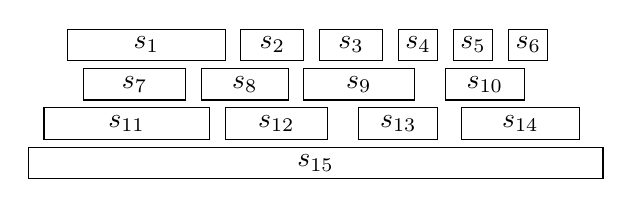
\begin{tikzpicture}
                \draw (0,4) rectangle node{$s_1$} (2,3.6);
                \draw (2.2,4) rectangle node{$s_2$} (3,3.6);
                \draw (3.2,4) rectangle node{$s_3$} (4,3.6);
                \draw (4.2,4) rectangle node{$s_4$} (4.7,3.6);
                \draw (4.9,4) rectangle node{$s_5$} (5.4,3.6);
                \draw (5.6,4) rectangle node{$s_6$} (6.1,3.6);

                \draw (0.2,3.5) rectangle node{$s_7$} (1.5,3.1);
                \draw (1.7,3.5) rectangle node{$s_8$} (2.8,3.1);
                \draw (3,3.5) rectangle node{$s_9$} (4.4,3.1);
                \draw (4.8,3.5) rectangle node{$s_{10}$} (5.8,3.1);

                \draw (-0.3,3) rectangle node{$s_{11}$} (1.8,2.6);
                \draw (2,3) rectangle node{$s_{12}$} (3.3,2.6);
                \draw (3.7,3) rectangle node{$s_{13}$} (4.7,2.6);
                \draw (5,3) rectangle node{$s_{14}$} (6.5,2.6);

                \draw (-0.5,2.5) rectangle node{$s_{15}$} (6.8,2.1);
            \end{tikzpicture}
        \end{center}
        \item Verwende den gierigen Algorithmus aus der Vorlesung, um für die folgenden Präferenzen ein stabiles Matching zu bestimmen:
        \begin{center}
            \begin{tabular}{c|c|c|c}
                x & y & z & w \\ \hline
                A & C & A & B \\
                C & D & D & C \\
                D & A & B & D \\
                B & B & C & A \\
            \end{tabular}
            \hspace{1cm}
            \begin{tabular}{c|c|c|c}
                A & B & C & D \\ \hline
                y & x & y & z \\
                x & z & w & w \\
                w & w & z & y \\
                z & y & x & x \\
            \end{tabular}
        \end{center}
    \end{enumerate}
\end{aufgabe}

\section*{Donnerstag}
\begin{aufgabe}[Antipathien]
    In der Algorithmen-Bank gab es während der Betriebsfeier viele Streitigkeiten zwischen den Angestellten. Daher wurde nach der Betriebsfeier ein Antipathie-Graph $G=(V,E)$ erstellt, in dem jede:r Angestellte durch einen Knoten der Menge $V=\{v_1,\ldots , v_n\}$ dargestellt wird. Eine ungerichtete Kante zwischen zwei Knoten bedeutet, dass sich diese beiden Angestellten nicht leiden können.\\
    Nun möchte man einen neuen Standort eröffnen. Um das Konkurrenzdenken zwischen den Standorten zu verstärken, möchte man die Angestellten in zwei Gruppen aufteilen, sodass die Anzahl an Antipathien (Kanten) zwischen den Gruppen maximal ist.\\
    Zur Bestimmung dieser Gruppen schlägt der Angestellte Aglot den folgenden gierigen Algorithmus vor:
    \begin{enumerate}
        \item[1.] Weise $v_1$ der Menge $A$ zu.
        \item[2.] für $i=2,\ldots , n$:
        \begin{itemize}
            \item[] Seien $a_i$ und $b_i$ die Anzahlen der Nachbarn von $v_i$ die bereits in $A$ oder $B$ sind
            \item[] Weise $v_i$ der Menge $A$ zu, wenn $a_i \leq b_i$ sonst weise $v_i$ der Menge $B$ zu 
        \end{itemize}
    \end{enumerate}
    \textbf{Zeige} oder \textbf{widerlege} folgende Aussagen:
    \begin{enumerate}[label=(\alph*)]
        \item Der gierige Algorithmus arbeitet optimal
        \item Der gierige Algorithmus kann mit Laufzeit $\mathcal{O}(n+m)$ implementiert werden, sofern $G$ in Adjazenzlistendarstellung gegeben ist.
        \item Der gierige Algorithmus findet eine Gruppenkonstellation mit mindestens $\frac{|E|}{2}$ Kanten zwischen den Gruppen.
    \end{enumerate}
\end{aufgabe}

\begin{aufgabe}[Balance II]
    % erickson 1st edition, June 2019; chp. 4 (greedy algorithms); ex. 22 b)
    \newcommand{\obr}{\textcolor{blue}{\texttt (}}
    \newcommand{\cbr}{\textcolor{red}{\texttt )}}
    Wir erinnern uns zurück an die \emoji{star}-Aufgabe von Woche 4 (``Balance'').
    Diesmal betrachten wir Strings mit nur einem Klammertyp.
    Ein String $w$ von Klammern \obr\ und \cbr\ ist \emph{balanciert}, wenn er eine der folgenden Bedingungen erfüllt:
    \begin{itemize}
        \item $w$ ist der leere String
        \item $w = \obr x \cbr$ für einen balancierten String $x$
        \item $w = xy$ für balancierte Strings $x$ und $y$.
    \end{itemize}
    Beispielsweise ist der String \obr \obr \cbr \cbr \obr \obr \obr \cbr \obr \cbr \cbr \cbr\ balanciert, während weder \obr \cbr \cbr, noch \obr \cbr \cbr \obr\ balanciert sind.

    \textbf{Beschreibe} einen gierigen Algorithmus mit Laufzeit $\mathcal O(n)$, welcher die Länge eines längsten balancierten Teilstrings in einem String der Länge $n$ berechnet.
    Dein Algorithmus soll ein Feld $w[1..n]$ entgegennehmen, wobei für jeden Index $i$ entweder $w[i] = \obr$ oder $w[i] = \cbr$ gilt.

    \emph{Hinweis: Welche elementare Datensturktur wurde damals in der \emoji{star}-Aufgabe verwendet?}
\end{aufgabe}

\begin{aufgabe}[Schuldenerlass]
    Aglot aus der Algorithmen-Bank schuldet seiner Kollegin Aifos 500.000€. Zum Erlassen seiner Schulden bietet sie Aglot folgenden Deal an:

    In einem blickdichten Beutel befindet sich eine Murmel, die entweder rot oder blau ist.
    Aglot kennt die Farbe der Murmel nicht, er weiß lediglich, dass beide Farben mit gleicher Wahrscheinlichkeit auftreten.
    Nun legt Aifos eine rote Murmel in den Beutel und schüttelt diesen einmal durch.
    Anschließend zieht sie rein zufällig eine Murmel aus dem Beutel und teilt Aglot die Farbe der gezogenen Murmel mit.
    Nun muss Aglot die Farbe der im Beutel verbliebenen Murmel erraten.
    Liegt er richtig, erlässt Aifos seine Schulden, andernfalls werden die Schulden verdoppelt.

    Selbstverständlich nimmt Aglot den Deal an.
    Aifos legt die rote Murmel in den Beutel, mischt einmal durch, und zieht anschließend eine rote Murmel aus dem Beutel.
    Welche Farbe sollte Aglot nun raten?
\end{aufgabe}

\end{document}
